

\section{Introduction}
% Vague bullshit
This is the collision detection group's final submission for the course TDT4295 Computer Design Project 2018. This course aims to give students an introduction to the process of designing physical computer solutions, from start to finish. The project was completed on a budget of 10000 NOK, of which 5400 NOK were spent. 

\subsection{What is BRICOLEUR?}

A bricoleur is someone who starts building something with no clear plan, adding bits here and there, cobbling together a whole while flying by the seat of their pants. 

The overarching goal of the project was to develop a stationary system which is able to detect moving objects, estimate their velocity and direction of motion, and finally predict a potential collision. In order to create concrete requirements for the minimum viable product, this was further reduced to the system being able to "predict collision with a single high-contrast object of reasonable size, moving in a straight line, and going no faster than 20 \sfrac{m}{s}".

\subsubsection{Additional requirements}
In addition to solving the problem described above, the project was to follow these constraints: 
\begin{itemize}
    \item The FPGA on the PYNQ must be used to perform meaningful acceleration of calculations. 
    \item The system must make use of a custom printed circuit board, which houses a micro control unit that is actively involved in the problem's solution. 
\end{itemize}

\subsection{Basic outline of solution}
The solution makes use of one camera and multiple ultrasonic sensors to detect incoming objects. The main code runs in Python on the PYNQ CPU, and is receiving images from the accelerator implemented on the FPGA. When the CPU has detected an incoming object it will send a signal to the microprocessor on the PCB that something is incoming. The ultrasonic sensors report directly to the microprocessor. The microprocessor will then output a byte value on UART, which indicates how sure it is that the object will collide both from the data from the CPU and from the ultrasonic sensors. 

\begin{figure}
    \centering
    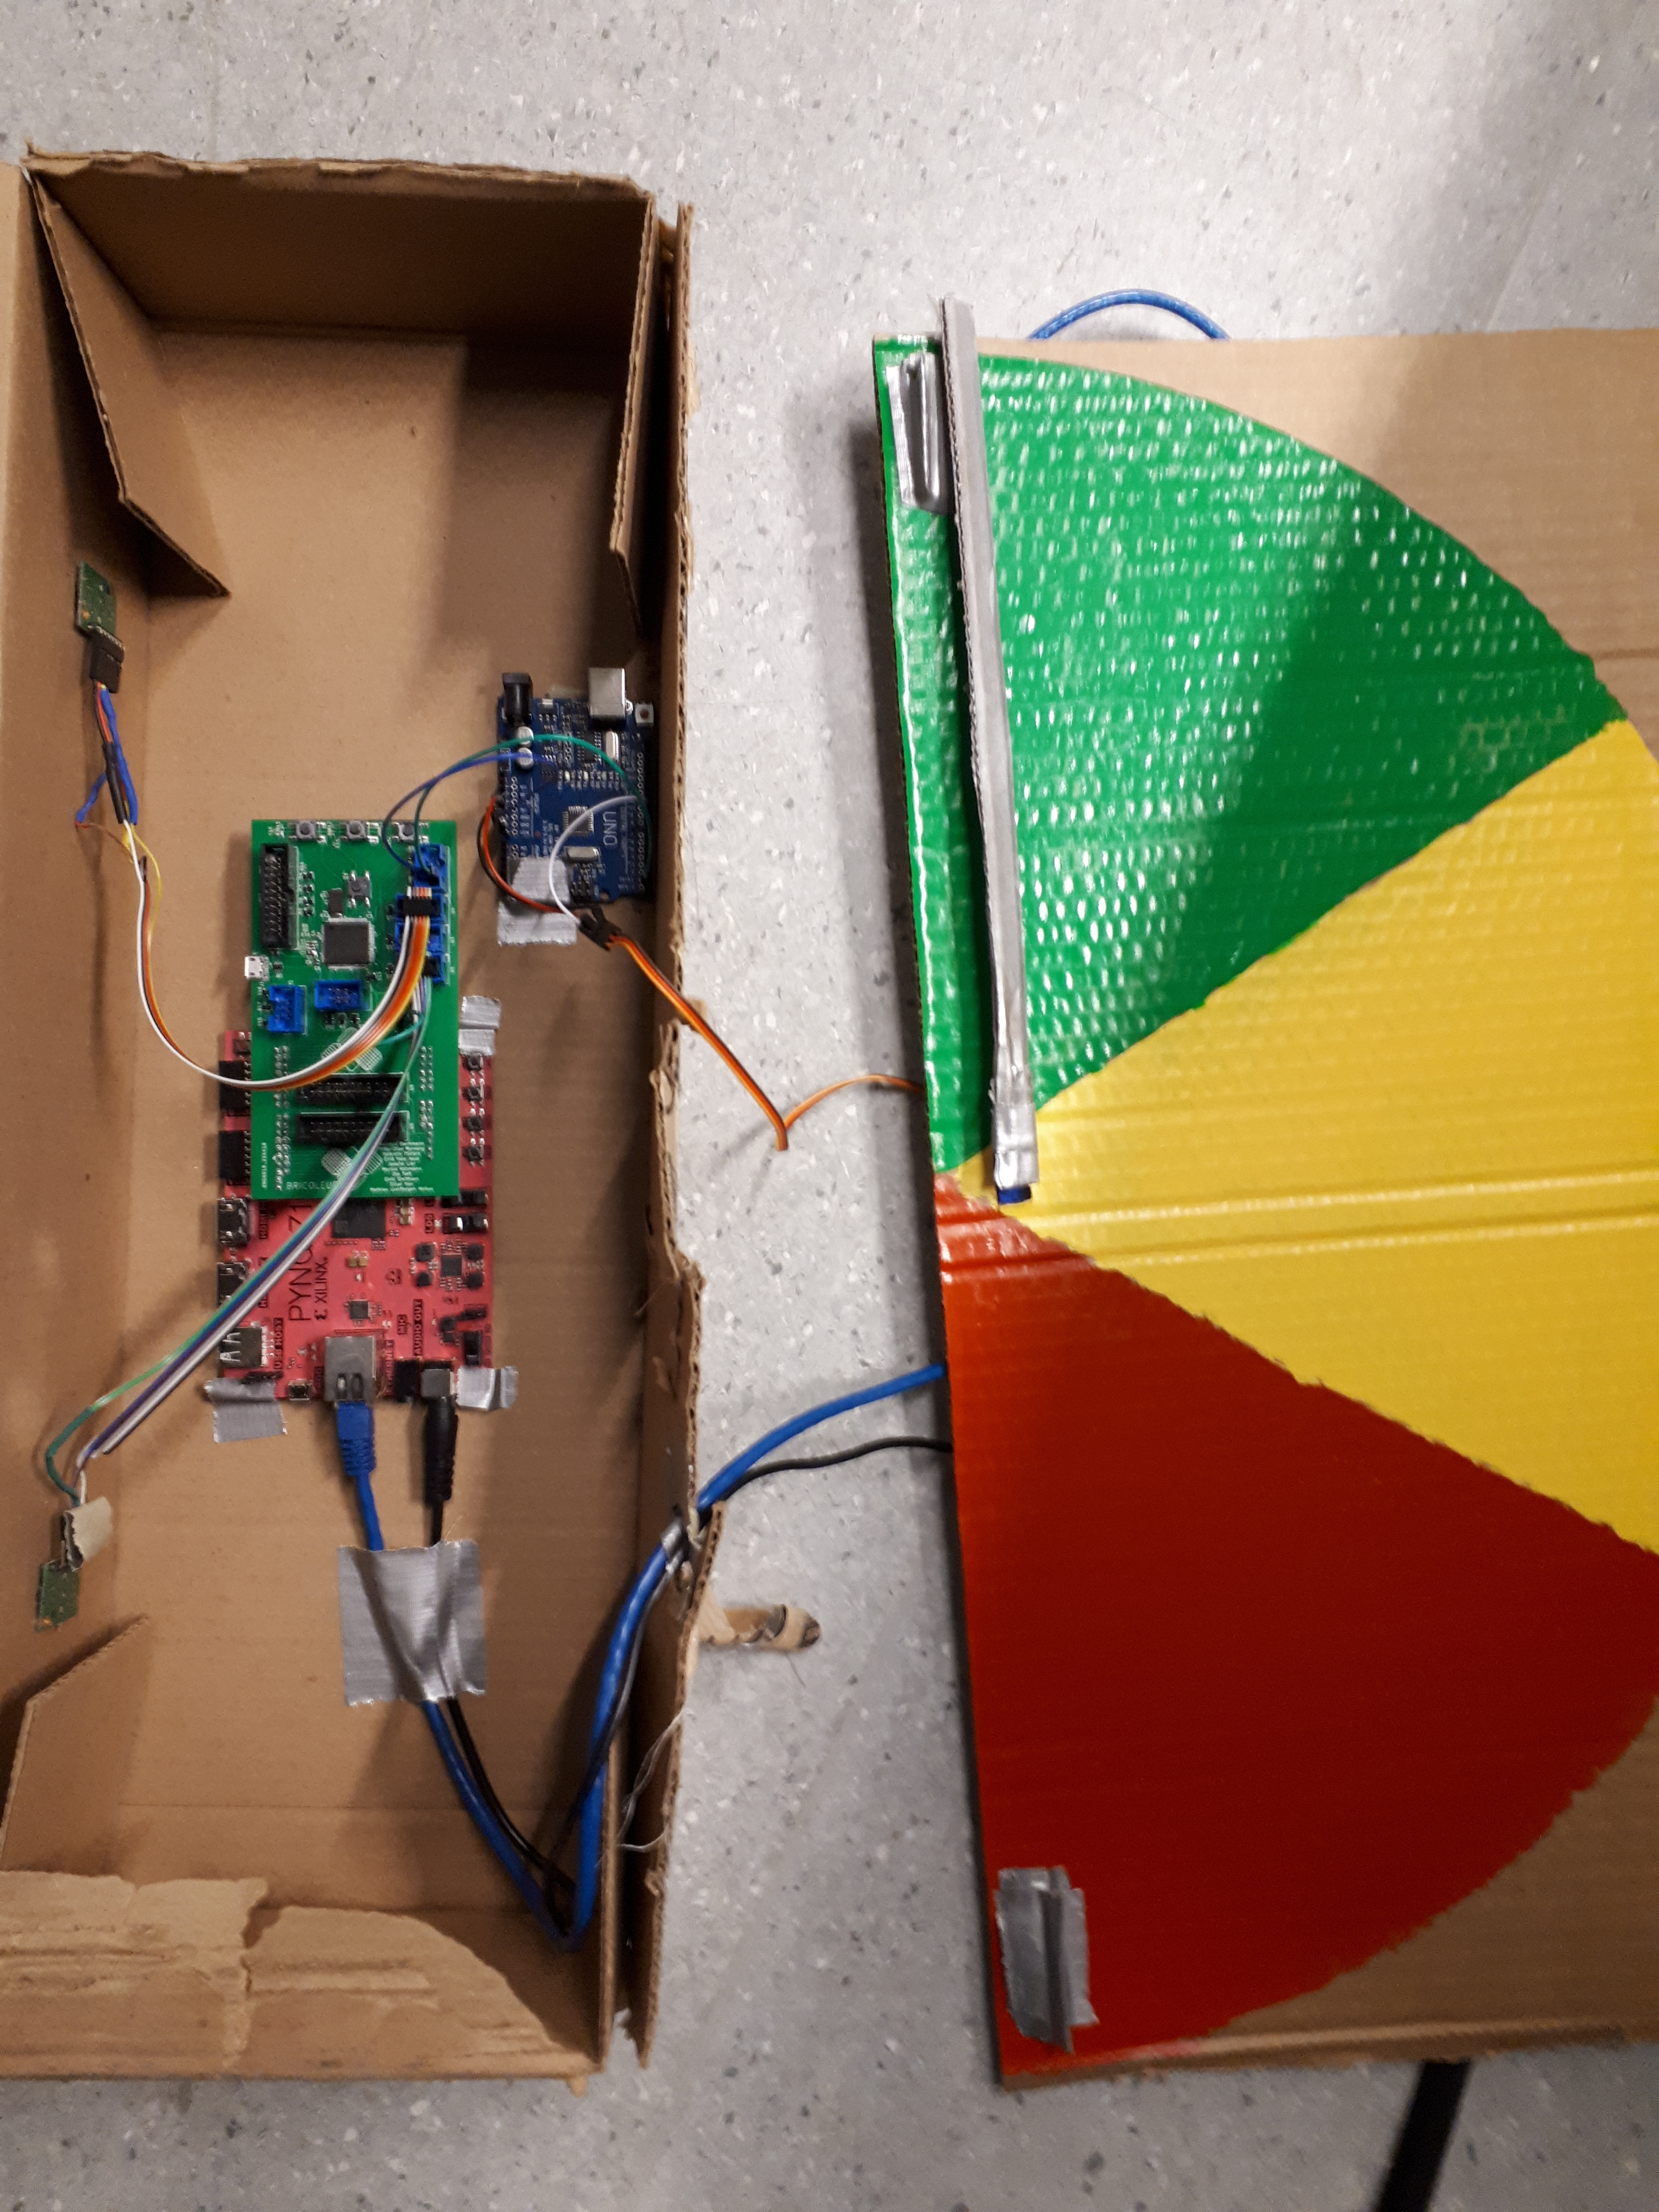
\includegraphics[scale=0.05]{Images/BRICOLEUR_FINAL.jpg}
    \caption{The contents of the final deliverable}
    \label{fig:finito}
\end{figure}